\documentclass[class=article, crop=false]{standalone}
\usepackage{my_preamble}
\begin{document}
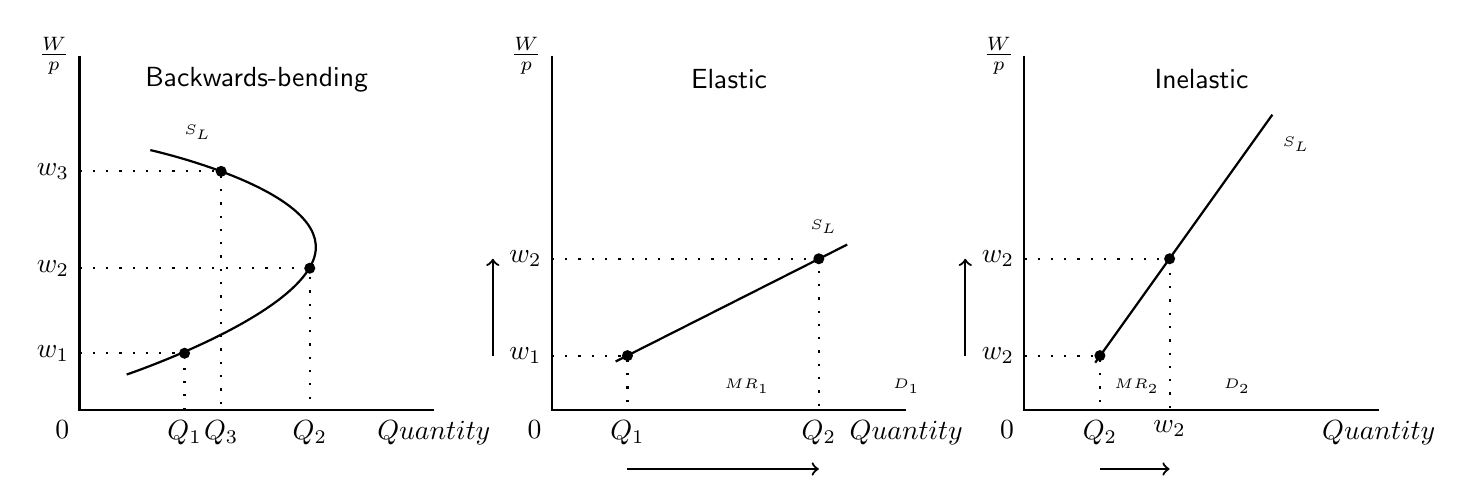
\begin{tikzpicture}[thick,font=\sffamily,scale=1.5]
	%axies
	\draw (-6,3) node[left]{$\frac{W}{p}$} -- (-6,0) node[below left] {$0$} -- (-3,0) node[below]{$Quantity$}; %market
	\draw (-2,3) node[left]{$\frac{W}{p}$} -- (-2,0) node[below left] {$0$} -- (1,0) node[below]{$Quantity$}; %type 1
	\draw (2,3) node[left]{$\frac{W}{p}$} -- (2,0) node[below left] {$0$} -- (5,0) node[below]{$Quantity$}; %type 2
	
	%titles
	\node[] at (-4.5,2.8) {Backwards-bending}; %Market title
	\node[] at (-0.5,2.8) {Elastic}; %Type 1 title
	\node[] at (3.5,2.8) {Inelastic}; %Market title
	  
	 %Backwards-bending D----------------------------------------------
	\node[right] at (-5.2,2.35) {\tiny{$S_{L}$}}; %Labour Supply label
	\draw[] plot [smooth, tension=1] coordinates {(-5.6,0.3) (-4,1.35) (-5.4,2.2)}; %Labour Supply
		%wage 1
		\node[style={fill=black,circle,inner sep=0pt,minimum size=4pt}] at (-5.11,0.48) { }; %node 1
		\draw[loosely dotted] (-6,0.48) node[left]{$w_{1}$} -| node[pos=0.25,below=3mm] {} (-5.11,0) node[below]{$Q_{1}$}; %dotted lines 1
		
		%wage 2
		\node[style={fill=black,circle,inner sep=0pt,minimum size=4pt}] at (-4.05,1.2) { }; %node 2
		\draw[loosely dotted] (-6,1.2) node[left]{$w_{2}$} -| node[pos=0.25,below=3mm] {} (-4.05,0) node[below]{$Q_{2}$}; %dotted lines 2
		
		%wage 3
		\node[style={fill=black,circle,inner sep=0pt,minimum size=4pt}] at (-4.8,2.02) { }; %node 3
		\draw[loosely dotted] (-6,2.02) node[left]{$w_{3}$} -| node[pos=0.25,below=3mm] {} (-4.8,0) node[below]{$Q_{3}$}; %dotted lines 3
	
	
	%Type 1 - elastic-------------------------------------
	\draw[] (-1.46,0.41) -- (0.5,1.4); %Elastic labour supply
	\node[right] at (0.1,1.55) {\tiny{$S_{L}$}}; %Labour Supply label
	\node[] at (1,0.2) {\tiny{$D_{1}$}}; %Demand1 label
	\node[] at (-0.35,0.2) {\tiny{$MR_{1}$}}; %MR1 label
	\node[style={fill=black,circle,inner sep=0pt,minimum size=4pt}] at (-1.36,0.46) { }; %mc=mr node
	\draw[loosely dotted] (-2,0.46) node[left]{$w_{1}$} -| node[pos=0.25,below=3mm] {} (-1.36,0) node[below]{$Q_{1}$}; %dotted lines
	
		%second wage
		\node[style={fill=black,circle,inner sep=0pt,minimum size=4pt}] at (0.26,1.28) { }; %node 2
		\draw[loosely dotted] (-2,1.28) node[left]{$w_{2}$} -| node[pos=0.25,below=3mm] {} (0.26,0) node[below]{$Q_{2}$}; %dotted lines 2
		
		%arrows
		\draw [->] (-1.36,-0.5) -- (0.26,-0.5); %x arrow
		\draw [->] (-2.5,0.46) -- (-2.5,1.28); %y arrow

	 
	%Type 2 - inelastic-----------------------------------
	\draw[] (2.6,0.4) -- (4.1,2.5); %Elastic labour supply
	\node[right] at (4.1,2.25) {\tiny{$S_{L}$}}; %Labour Supply label
	\node[] at (3.8,0.2) {\tiny{$D_{2}$}}; %Demand2 label
	\node[] at (2.95,0.2) {\tiny{$MR_{2}$}}; %MR2 label
	\node[style={fill=black,circle,inner sep=0pt,minimum size=4pt}] at (2.64,0.46) { }; %mc=mr node
	\draw[loosely dotted] (2,0.46) node[left]{$w_{2}$} -| node[pos=0.25,below=3mm] {} (2.64,0) node[below]{$Q_{2}$}; %dotted lines
	
		%second wage
		\node[style={fill=black,circle,inner sep=0pt,minimum size=4pt}] at (3.23,1.28) { }; %node 2
		\draw[loosely dotted] (2,1.28) node[left]{$w_{2}$} -| node[pos=0.25,below=3mm] {} (3.23,0) node[below]{$w_{2}$}; %dotted lines 2
		
		%arrows
		\draw [->] (2.64,-0.5) -- (3.23,-0.5); %x arrow
		\draw [->] (1.5,0.46) -- (1.5,1.28); %y arrow
		
\end{tikzpicture}
\end{document}